\subsection{UC16 - Telegram - Interazioni}
		
		%\begin{figure}[t!]
		%	\centering
		%	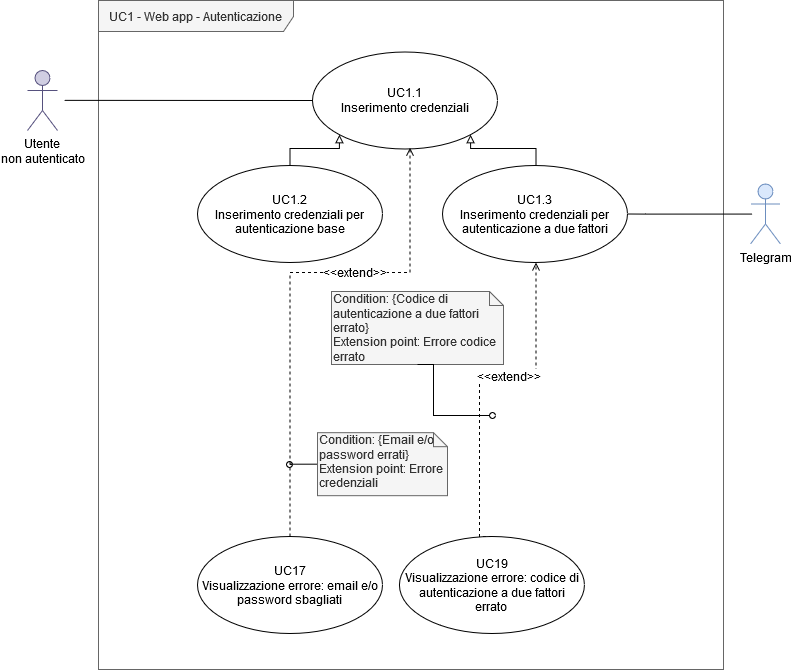
\includegraphics[height=10em]{res/images/uc1}
		%\end{figure}
		
	\begin{itemize}
		\item \textbf{Attori Primari}: Utente autenticato, Moderatore Ente.
		\item \textbf{Attori Secondari}: \glock{Telegram}.
		\item \textbf{Descrizione}: L'utente mentre è nell'applicazione di \glock{Telegram} può eseguire delle interazioni per gestire dispositivi remoti nel sistema o ricevere informazioni particolari. 
		\item \textbf{Precondizione}: L'utente sta usando l'applicazione di \glock{Telegram} e ha eseguito l'autenticazione.
		\item \textbf{Postcondizione}: L'utente riceve un messaggio di risposta dal \glock{Bot} di \glock{Telegram}.
		\item \textbf{Scenario Principale}:
		\begin{enumerate}
			\item L'utente esegue una interazione con il \glock{Bot} di \glock{Telegram}.
		\end{enumerate}
	\end{itemize}
	
	\subsubsection{UC 16.1 - Interazione con comando}

	\begin{itemize}
		\item \textbf{Attori Primari}: Utente autenticato, Moderatore Ente.
		\item \textbf{Attori Secondari}: \glock{Telegram}.
		\item \textbf{Descrizione}: L'utente esegue una interazione con \glock{Telegram} e riceve una risposta in base al comando che ha inviato. 
		\item \textbf{Precondizione}: L'utente sta usando l'applicazione di \glock{Telegram}.
		\item \textbf{Postcondizione}: L'utente riceve un messaggio di risposta dopo aver eseguito una interazione con \glock{Telegram}.
		\item \textbf{Scenario Principale}:
		\begin{enumerate}
			\item L'utente sta usando l'applicazione di \glock{Telegram} e ha una chat aperta e autenticata con il bot. 
			\item L'utente esegue una interazione con \glock{Telegram}.
			\item L'utente riceve dei messaggi di risposta da parte del \glock{Bot} di \glock{Telegram}.
		\end{enumerate}
		\item \textbf{Specializzazioni}:
		\begin{itemize}
			\item Comando di inizio (UC 16.1.1);
			\item Comando per le informazioni (UC 16.1.2);
			\item Comando per l'aiuto (UC 16.1.3);
			\item Comando di interazione con i dispositivi (UC 16.1.4).
		\end{itemize}
		\item \textbf{Estensioni}:
		\begin{itemize}
			\item Nessuna risposta dopo una interazione con Telegram (UC 20).
		\end{itemize}
	\end{itemize}

	\subsubsection{UC 16.2 - Comando di inizio}

	\begin{itemize}
		\item \textbf{Attori Primari}: Utente autenticato.
		\item \textbf{Attori Secondari}: \glock{Telegram}.
		\item \textbf{Descrizione}: L'utente esegue una interazione con il comando di inizio per recuperare le informazioni sull'autenticazione.
		\item \textbf{Precondizione}: L'utente sta usando l'applicazione di \glock{Telegram}.
		\item \textbf{Postcondizione}: L'utente ha eseguito una interazione con \glock{Telegram}.
		\item \textbf{Scenario Principale}:
		\begin{enumerate}
			\item L'utente sta usando l'applicazione di \glock{Telegram}. 
			\item L'utente invia il comando (UC 16.2.1).
		\end{enumerate}
	\end{itemize}

		\paragraph{UC 16.2.1 - Invio comando}
		\begin{itemize}
			\item \textbf{Attori Primari}: Utente autenticato.
			\item \textbf{Attori Secondari}: \glock{Telegram}.
			\item \textbf{Descrizione}: L'utente invia il comando di inizio nell'applicazione \glock{Telegram}.
			\item \textbf{Precondizione}: L'utente sta usando l'applicazione di \glock{Telegram}.
			\item \textbf{Postcondizione}: L'utente ha eseguito una interazione da \glock{Telegram}.
			\item \textbf{Scenario Principale}:
			\begin{enumerate}
				\item L'utente invia il comando di inizio al \glock{Bot} di \glock{Telegram}.
			\end{enumerate}
			\item \textbf{Inclusioni}:
			\begin{enumerate}
				\item L'utente riceve un messaggio di ritorno da \glock{Telegram} (UC 16.2.2).
			\end{enumerate}
		\end{itemize}

		\paragraph{UC 16.2.2 - Messaggio di ritorno}
		\begin{itemize}
			\item \textbf{Attori Primari}: Utente autenticato.
			\item \textbf{Attori Secondari}: \glock{Telegram}.
			\item \textbf{Descrizione}: L'utente riceve un messaggio di ritorno su \glock{Telegram}, dopo aver inviato il comando, illustrando le informazioni dell'account autenticato.
			\item \textbf{Precondizione}: L'utente sta usando l'applicazione di \glock{Telegram}.
			\item \textbf{Postcondizione}: L'utente ha eseguito una interazione da \glock{Telegram}.
			\item \textbf{Scenario Principale}:
			\begin{enumerate}
				\item L'utente riceve un messaggio al \glock{Bot} di \glock{Telegram}.
			\end{enumerate}
		\end{itemize}


	\subsubsection{UC 16.1 - Interazione con comando}

	\begin{itemize}
		\item \textbf{Attori Primari}: Utente autenticato, Moderatore Ente.
		\item \textbf{Attori Secondari}: \glock{Telegram}.
		\item \textbf{Descrizione}: L'utente esegue una interazione con \glock{Telegram} e riceve una risposta in base al comando che ha inviato. 
		\item \textbf{Precondizione}: L'utente sta usando l'applicazione di \glock{Telegram}.
		\item \textbf{Postcondizione}: L'utente riceve un messaggio di risposta dopo aver eseguito una interazione con \glock{Telegram}.
		\item \textbf{Scenario Principale}:
		\begin{enumerate}
			\item L'utente sta usando l'applicazione di \glock{Telegram} e ha una chat aperta e autenticata con il bot. 
			\item L'utente esegue una interazione con \glock{Telegram}.
			\item L'utente riceve dei messaggi di risposta da parte del \glock{Bot} di \glock{Telegram}.
		\end{enumerate}
		\item \textbf{Specializzazioni}:
		\begin{itemize}
			\item Comando di inizio (UC 16.1.1);
			\item Comando per le informazioni (UC 16.1.2);
			\item Comando per l'aiuto (UC 16.1.3);
			\item Comando di interazione con i dispositivi (UC 16.1.4).
		\end{itemize}
		\item \textbf{Estensioni}:
		\begin{itemize}
			\item Nessuna risposta dopo una interazione con Telegram (UC 20).
		\end{itemize}
	\end{itemize}


	\subsubsection{UC 16.3 - Comando di informazioni}
	\begin{itemize}
		\item \textbf{Attori Primari}: Utente autenticato.
		\item \textbf{Attori Secondari}: \glock{Telegram}.
		\item \textbf{Descrizione}: L'utente esegue una interazione con il comando di \textit{informazioni} per recuperare la versione del bot, le info del sistema e l'account con cui si è autenticati.
		\item \textbf{Precondizione}: L'utente ha iniziato a interagire con \glock{Telegram}.
		\item \textbf{Postcondizione}: L'utente ha eseguito una interazione con \glock{Telegram}.
		\item \textbf{Scenario Principale}:
		\begin{enumerate}
			\item L'utente sta usando l'applicazione di \glock{Telegram}. 
			\item L'utente invia il comando (UC 16.3.1).
		\end{enumerate}
	\end{itemize}

		\paragraph{UC 16.3.1 - Invio comando}
		\begin{itemize}
			\item \textbf{Attori Primari}: Utente autenticato.
			\item \textbf{Attori Secondari}: \glock{Telegram}.
			\item \textbf{Descrizione}: L'utente invia il comando di \textit{informazioni} nell'applicazione \glock{Telegram}.
			\item \textbf{Precondizione}: L'utente sta usando l'applicazione di \glock{Telegram}.
			\item \textbf{Postcondizione}: L'utente ha eseguito una interazione da \glock{Telegram}.
			\item \textbf{Scenario Principale}:
			\begin{enumerate}
				\item L'utente invia il comando di \textit{informazioni} al \glock{Bot} di \glock{Telegram}.
			\end{enumerate}
			\item \textbf{Inclusioni}:
			\begin{enumerate}
				\item L'utente riceve un messaggio di ritorno da \glock{Telegram} (UC 16.3.2).
			\end{enumerate}
		\end{itemize}

		\paragraph{UC 16.3.2 - Messaggio di ritorno}
		\begin{itemize}
			\item \textbf{Attori Primari}: Utente autenticato.
			\item \textbf{Attori Secondari}: \glock{Telegram}.
			\item \textbf{Descrizione}: L'utente riceve un messaggio di ritorno su \glock{Telegram}, dopo aver inviato il comando, illustrante la versione del bot, le info del sistema e l'account con cui si è autenticati.
			\item \textbf{Precondizione}: L'utente ha iniziato a interagire con l'applicazione di \glock{Telegram}.
			\item \textbf{Postcondizione}: L'utente ha eseguito una interazione da \glock{Telegram}.
			\item \textbf{Scenario Principale}:
			\begin{enumerate}
				\item L'utente riceve un messaggio dal \glock{Bot} di \glock{Telegram}.
			\end{enumerate}
		\end{itemize}		


	\subsubsection{UC 16.4 - Comando per l'aiuto}
	\begin{itemize}
		\item \textbf{Attori Primari}: Utente autenticato.
		\item \textbf{Attori Secondari}: \glock{Telegram}.
		\item \textbf{Descrizione}: L'utente esegue una interazione con il comando di \textit{aiuto} per recuperare la lista dei comandi disponibili.
		\item \textbf{Precondizione}: L'utente ha iniziato a interagire con \glock{Telegram}.
		\item \textbf{Postcondizione}: L'utente ha eseguito una interazione con \glock{Telegram}.
		\item \textbf{Scenario Principale}:
		\begin{enumerate}
			\item L'utente sta usando l'applicazione di \glock{Telegram}. 
			\item L'utente invia il comando (UC 16.4.1).
		\end{enumerate}
	\end{itemize}

		\paragraph{UC 16.4.1 - Invio comando}
		\begin{itemize}
			\item \textbf{Attori Primari}: Utente autenticato.
			\item \textbf{Attori Secondari}: \glock{Telegram}.
			\item \textbf{Descrizione}: L'utente invia il comando di \textit{aiuto} nell'applicazione \glock{Telegram}.
			\item \textbf{Precondizione}: L'utente sta usando l'applicazione di \glock{Telegram}.
			\item \textbf{Postcondizione}: L'utente ha eseguito una interazione da \glock{Telegram}.
			\item \textbf{Scenario Principale}:
			\begin{enumerate}
				\item L'utente invia il comando di \textit{aiuto} al \glock{Bot} di \glock{Telegram}.
			\end{enumerate}
			\item \textbf{Inclusioni}:
			\begin{enumerate}
				\item L'utente riceve un messaggio di ritorno da \glock{Telegram} (UC 16.4.2).
			\end{enumerate}
		\end{itemize}

		\paragraph{UC 16.4.2 - Messaggio di ritorno}
		\begin{itemize}
			\item \textbf{Attori Primari}: Utente autenticato.
			\item \textbf{Attori Secondari}: \glock{Telegram}.
			\item \textbf{Descrizione}: L'utente riceve un messaggio di ritorno su \glock{Telegram}, dopo aver inviato il comando, illustrante la lista dei comandi disponibili con una relativa descrizione.
			\item \textbf{Precondizione}: L'utente ha iniziato a interagire con l'applicazione di \glock{Telegram}.
			\item \textbf{Postcondizione}: L'utente ha eseguito una interazione da \glock{Telegram}.
			\item \textbf{Scenario Principale}:
			\begin{enumerate}
				\item L'utente riceve un messaggio dal \glock{Bot} di \glock{Telegram}.
			\end{enumerate}
		\end{itemize}	


	\subsubsection{UC 16.5 - Comando di interazione con i dispositivi}
	\begin{itemize}
		\item \textbf{Attori Primari}: Moderatore ente.
		\item \textbf{Attori Secondari}: \glock{Telegram}.
		\item \textbf{Descrizione}: L'utente esegue una interazione per richiedere di visualizzare i dispositivi attivi e di inviare input a un dispositivo remoto. 
		\item \textbf{Precondizione}: L'utente ha iniziato a interagire con \glock{Telegram} e l'utente è autenticato come Moderatore ente.
		\item \textbf{Postcondizione}: L'utente ha eseguito una interazione con \glock{Telegram}.
		\item \textbf{Scenario Principale}:
		\begin{enumerate}
			\item L'utente sta usando l'applicazione di \glock{Telegram}.;
			\item L'utente invia il comando (UC 16.5.1).
		\end{enumerate}
		\item \textbf{Inclusioni}:
		\begin{itemize}
			\item L'utente riceve la lista dei dispositivi attivi (UC 16.5.2)
		\end{itemize}
	\end{itemize}


		\paragraph{UC 16.5.1 - Invio comando per la lista dispositivi}
		\begin{itemize}
			\item \textbf{Attori Primari}: Moderatore ente.
			\item \textbf{Attori Secondari}: \glock{Telegram}.
			\item \textbf{Descrizione}: L'utente invia il comando per lista dispositivi nell'applicazione \glock{Telegram}.
			\item \textbf{Precondizione}: L'utente sta usando l'applicazione di \glock{Telegram}.
			\item \textbf{Postcondizione}: L'utente ha eseguito una interazione da \glock{Telegram}.
			\item \textbf{Scenario Principale}:
			\begin{enumerate}
				\item L'utente invia il comando di per la lista dispositivi al \glock{Bot} di \glock{Telegram}.
			\end{enumerate}
			\item \textbf{Inclusioni}:
			\begin{enumerate}
				\item L'utente riceve una lista dei dispositivi da \glock{Telegram} (UC 16.5.2).
			\end{enumerate}
		\end{itemize}

		\paragraph{UC 16.5.2 - Ricezione lista dei dispositivi attivi}
		\begin{itemize}
			\item \textbf{Attori Primari}: Moderatore ente.
			\item \textbf{Attori Secondari}: \glock{Telegram}.
			\item \textbf{Descrizione}: L'utente riceve un messaggio di ritorno su \glock{Telegram}, dopo aver inviato il comando, illustrante la lista dei dispositivi remoti disponibili e pronti alla ricezione di un input. 
			\item \textbf{Precondizione}: L'utente ha iniziato a interagire con l'applicazione di \glock{Telegram} e ha inviato un comando.
			\item \textbf{Postcondizione}: L'utente ha eseguito una interazione da \glock{Telegram}.
			\item \textbf{Scenario Principale}:
			\begin{enumerate}
				\item L'utente riceve un messaggio dal \glock{Bot} di \glock{Telegram}.
			\end{enumerate}
		\end{itemize}	


		\paragraph{UC 16.5.3 - Invio comando di selezione del dispositivo}
		\begin{itemize}
			\item \textbf{Attori Primari}: Moderatore ente.
			\item \textbf{Attori Secondari}: \glock{Telegram}.
			\item \textbf{Descrizione}: L'utente invia il comando per la selezione di un dispositivo remoto nell'applicazione \glock{Telegram}.
			\item \textbf{Precondizione}: L'utente sta usando l'applicazione di \glock{Telegram}.
			\item \textbf{Postcondizione}: L'utente ha eseguito una interazione da \glock{Telegram}.
			\item \textbf{Scenario Principale}:
			\begin{enumerate}
				\item L'utente invia il comando di per la selezione di un dispositivo remoto al \glock{Bot} di \glock{Telegram}.
			\end{enumerate}
			\item \textbf{Inclusioni}:
			\begin{enumerate}
				\item L'utente riceve una lista degli input inviabili al dispositivo da \glock{Telegram} (UC 16.5.4).
			\end{enumerate}
		\end{itemize}

		\paragraph{UC 16.5.4 - Ricezione dei possibili comandi da inviare al dispositivo }
		\begin{itemize}
			\item \textbf{Attori Primari}: Moderatore ente.
			\item \textbf{Attori Secondari}: \glock{Telegram}.
			\item \textbf{Descrizione}: L'utente riceve un messaggio di ritorno su \glock{Telegram}, dopo aver inviato il comando, illustrante la lista degli input disponibili per un dato dispositivo richiesto. 
			\item \textbf{Precondizione}: L'utente ha iniziato a interagire con l'applicazione di \glock{Telegram} e ha inviato un comando.
			\item \textbf{Postcondizione}: L'utente ha eseguito una interazione da \glock{Telegram}.
			\item \textbf{Scenario Principale}:
			\begin{enumerate}
				\item L'utente riceve un messaggio dal \glock{Bot} di \glock{Telegram}.
			\end{enumerate}
		\end{itemize}	

		\paragraph{UC 16.5.5 - Invio comando al dispositivo}
		\begin{itemize}
			\item \textbf{Attori Primari}: Moderatore ente.
			\item \textbf{Attori Secondari}: \glock{Telegram}.
			\item \textbf{Descrizione}: L'utente invia il comando con un input per un dispositivo remoto preciso, nell'applicazione \glock{Telegram}.
			\item \textbf{Precondizione}: L'utente sta usando l'applicazione di \glock{Telegram}.
			\item \textbf{Postcondizione}: L'utente ha eseguito una interazione da \glock{Telegram}.
			\item \textbf{Scenario Principale}:
			\begin{enumerate}
				\item L'utente invia un comando di input per un dispositivo remoto al \glock{Bot} di \glock{Telegram}.
			\end{enumerate}
			\item \textbf{Inclusioni}:
			\begin{enumerate}
				\item L'utente riceve un messaggio di ritorno da \glock{Telegram} (UC 16.5.6).
			\end{enumerate}
		\end{itemize}

		\paragraph{UC 16.5.6 - Messaggio di ritorno }
		\begin{itemize}
			\item \textbf{Attori Primari}: Moderatore ente.
			\item \textbf{Attori Secondari}: \glock{Telegram}.
			\item \textbf{Descrizione}: L'utente riceve un messaggio di ritorno su \glock{Telegram}, dopo aver inviato il comando, che segnala l'invio corretto dell'input al dispositivo. 
			\item \textbf{Precondizione}: L'utente ha iniziato a interagire con l'applicazione di \glock{Telegram} e ha inviato un comando.
			\item \textbf{Postcondizione}: L'utente ha eseguito una interazione da \glock{Telegram}.
			\item \textbf{Scenario Principale}:
			\begin{enumerate}
				\item L'utente riceve un messaggio dal \glock{Bot} di \glock{Telegram}.
			\end{enumerate}
		\end{itemize}	

		




